W poprzedzających częściach pracy zakładaliśmy, że granice między ośrodkami tworzącymi wielowarstwę są idealnie płaskie. W warunkach eksperymentalnych, przy wykorzystaniu technik umożliwiających naprzemienne układanie kilkunastu warstw różnych materiałów o grubości od kilkunastu do kilkudziesięciu nanometrów,  takich jak fizyczne osadzanie z fazy gazowej (ang. PVD - physical vapour deposition), uzyskanie takich warstw jest niemożliwe. W poniższym rozdziale przeanalizowany zostanie wpływ niedoskonałości warstw na obrazowanie przez struktury MDM.

Podstawowym parametrem wykorzystywanym do opisu chropowatości jest średnia kwadratowa różnic faktycznej grubości warstwy od zamierzonej (ang. RMS - root mean squere). Różnice uzyskanej w stosunku do projektowanej grubości warstwy w kolejnych punktach nie tworzą zmiennej losowej o charakterystyce szumu białego, dlatego do pełnego opisu topologii powierzchni niezbędne jest wykorzystanie funkcji autokorelacji\cite{stefaniuk2011effect}. Na podstawie pomiarów mikroskopem sił atomowych (ang. AFM - atomic force microscope) można stwierdzić, że RMS powierzchni podlega statystyce Gaussowskiej. Histogram wyników uzyskanych przy pomocy pomiarów AFM prezentuje wykres \ref{fig:ag30nm-afmhist}, dwu wymiarowy skan uzyskany w pomiarach prezentuje rysunek \ref{fig:ag30nm-afmmeasure}.

\begin{figure}[bt]
		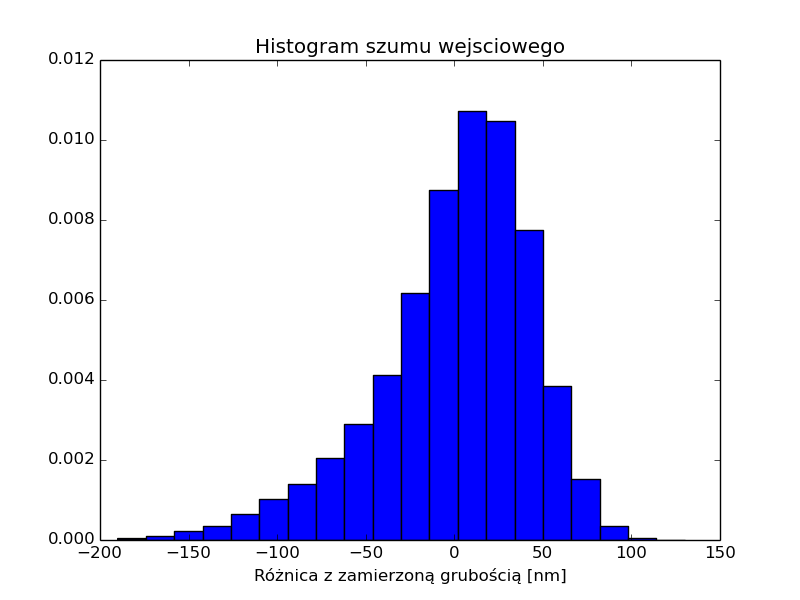
\includegraphics[width=\textwidth]{images/multilayer/ag30nm-afm-measure-hist.png}
		\caption{Histogram odchyleń od zamierzonej grubości dla warstwy $30$~nm obserwowanej przy pomocy AFM w punktach odległych od siebie o $11.7$~nm} 		\label{fig:ag30nm-afmhist}
\end{figure}

\begin{figure}[bt]
		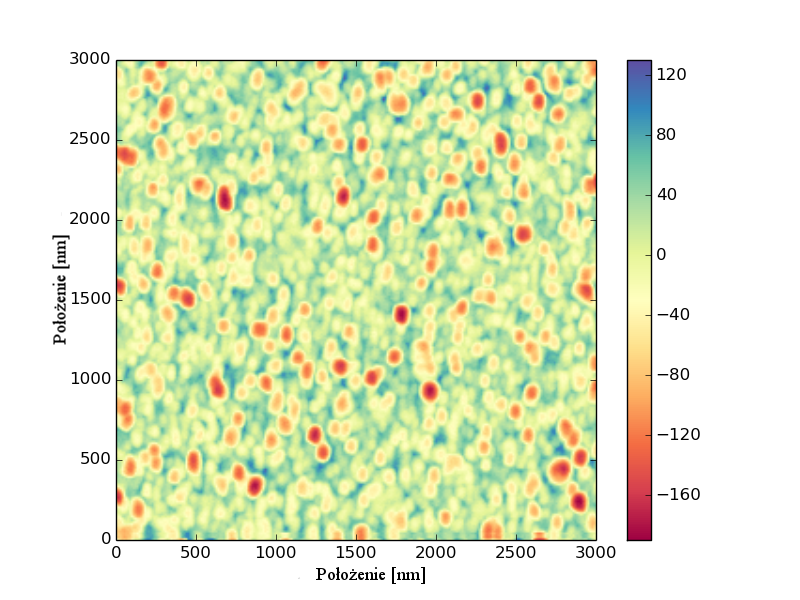
\includegraphics[width=\textwidth]{images/multilayer/ag30nm-afm-measure.png}
		\caption{Pomiary grubości na powierzchni napylonej warstwy $30$~nm srebra za pomocą AFM} 
		\label{fig:ag30nm-afmmeasure}
\end{figure}


Efektywne współczynniki przenikalności elektrycznej uzyskiwane przy pomocy \ref{eq:effmedium} w znacznym stopniu zmieniają się w wyniku wprowadzenia chropowatości. Szczególnie dużą zmienność można zaobserwować w okolicach rezonansu dyspersyjnego dla $\varepsilon_{\perp}$, czyli w zakresie długości fali dla którego projektowane są własności metamateriału.  Zbliżenie wartości do przewiydywanych w warunkach homogenizacji można zaobserwować w przypadku symulacji struktur dla których na większych obszarach zadano gładką zmienność grubości warstwy. W ten sposób otrzymując większe gładkie obszary na powierzchni symulowanej granicy między ośrodkami \cite{ludwig2012impact}. 

\begin{figure}[!hbt]
	\begin{center}
	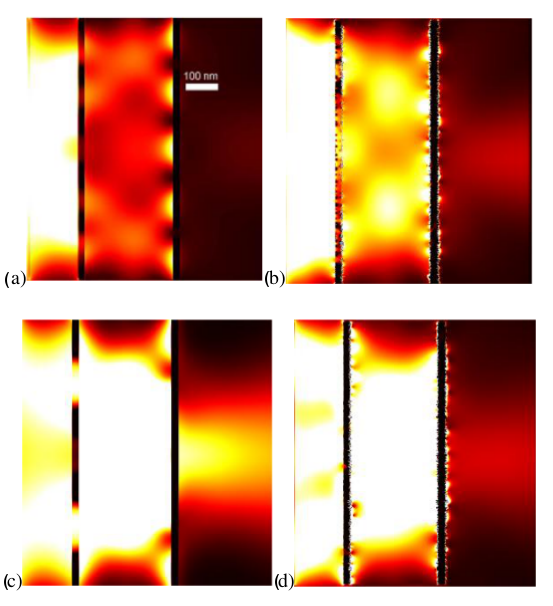
\includegraphics[width=.9\textwidth]{images/multilayer/plp-chropo.png}
	\end{center}
	\caption{Rozkład natężenia polal ektromagnetycznego wewnątrz i poza strukturą warstwową o własnościach supersoczewki z warstwami chropowatymi, oświetloną przy pomocy źródła monochromatycznego o długościach fali odpowiednio a,b $\lambda=430$~nm  i  c,d $\lambda=490$~nm~\cite{Stolarek_2013}}
	\label{fig:plp-chropo-fdtd}
\end{figure}


Analizując włściwości obrazujące wielowarstw metaliczno-dielektrycznych należy również zwrócić uwagę, że wprowadznie chropowatości może mieć pozytywny wpływ. Wprowadzenie chropowatości może zwiększyć współczynnik transmisji przez granicę dwuch ośrodków poprzez skrócenie zasięgu propagacji plazmonów powierzchniowych \cite{huang2012subwavelength}. Przykład układu dla którego wprowadzenie chropowatości zwiększa współczynnik transmisji przez układ dla wąskiego zakresu długości fali prezentuje rozkład pola elektromagnetycznego na rysunku \ref{fig:plp-chropo-fdtd} a i b. W ogólności jednak wzrost chropowatości powierzchni zmniejsza współczynnik transmisji przez strukturę warstwową, co możemy zaobserwować po zmiane długości fali oświetlającej soczewkę na rozkładach pola na rysunkach \ref{fig:pl-chropo-fdtd} c i d. 

\begin{figure}[bt]
		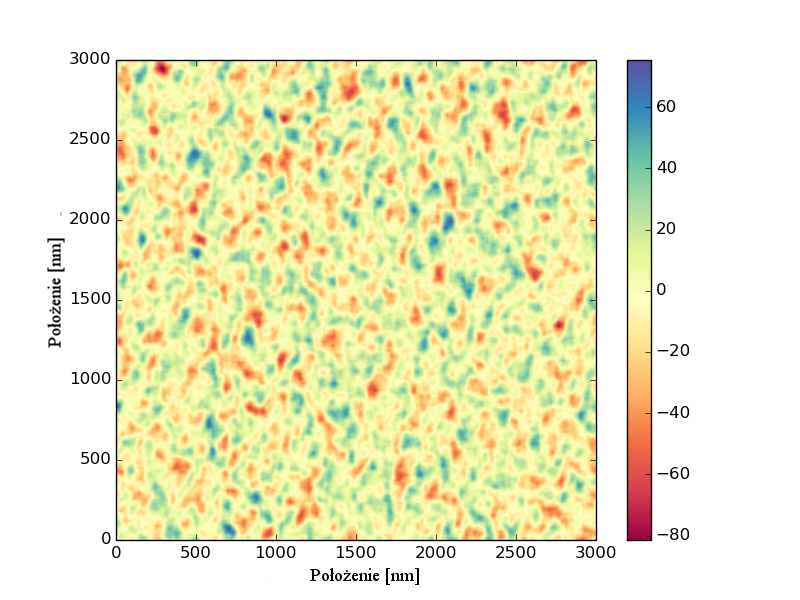
\includegraphics[width=\textwidth]{images/multilayer/ag30nm-afm-generated.png}
		\caption{Wizualizacja powierzchni chropowatej wygenerwowanej na podstawie pomiarów AFM. Generowana jest zmienna losowa podlegające rozkładowi normalnemu o widmowej gęstości mocy odpowiadającej wyniokom pomiarów przy pomocy AFM.} 
		\label{fig:ag30nm-afmgene}
%	Generator:
%	pomocnicze/wielowarstw/chropo/gen-chropo.py
\end{figure}


Zmiana właściwosći materiałów budujących wielowarstwę na charakteryzujące się mniejszą absorpcją nie może skompensować tego zjawiska. Wprowadzenie chropowatości warstw prowadzi do powstania losowych zaburzeń rozkładu pola elektromagnetycznego, których interferencja wprowadza zniekształcenie optycznej funkcji przenoszenia(ang. OTF - Optical Transfer Function). Odpowiednio dobrany współczynnik absorpcji wewnątrz metali zapewnia szybkie zanikanie losowych zaburzeń umożliwiając zachowanie płaskiego charakteru OTF. Szczególne znaczenie dla zachowania własności obrazowania podfalowego ma płaszczyzna wyjściowa wielowarstwy, na której utrzymanie RMS poniżej $0.6$~nm jest kluczowe dla uzyskania PSF o szerokości podfalowej. \cite{guo2014negative}

Należy zwrócić uwagę, że na skutek chropowatości współczynnik $\varepsilon_{\perp}$ zostaje zmniejszony w okolicach rezonansu (dla idealnej supersoczewki $\varepsilon_{\perp} \to - \infty$), co powoduje, że możliwa jest efektywna transmisja wyższych częstości przestrzennych a co za tym idzie zwiększenie zdolności rozdzielczej układu. Własności obrazujące, które byłby optymalne przy płaskim kształcie OTF zostają jednocześnie zaburzone, a ich zachowanie możliwe jest poprzez użycie materiałów o większym współczynniku absorpcji. Na podstawie takiego rozważania Zhen Guo i in. wnioskują, że chropowatośc w zasadniczy sposób pogarsza zdolności obrazujące supersoczewki, zdolności rozdzielcza jest natomiast kontrolowana poprzez stratność użytych materiałów.

\begin{figure}
	\centering
	\begin{subfigure}[b]{.45\textwidth}
		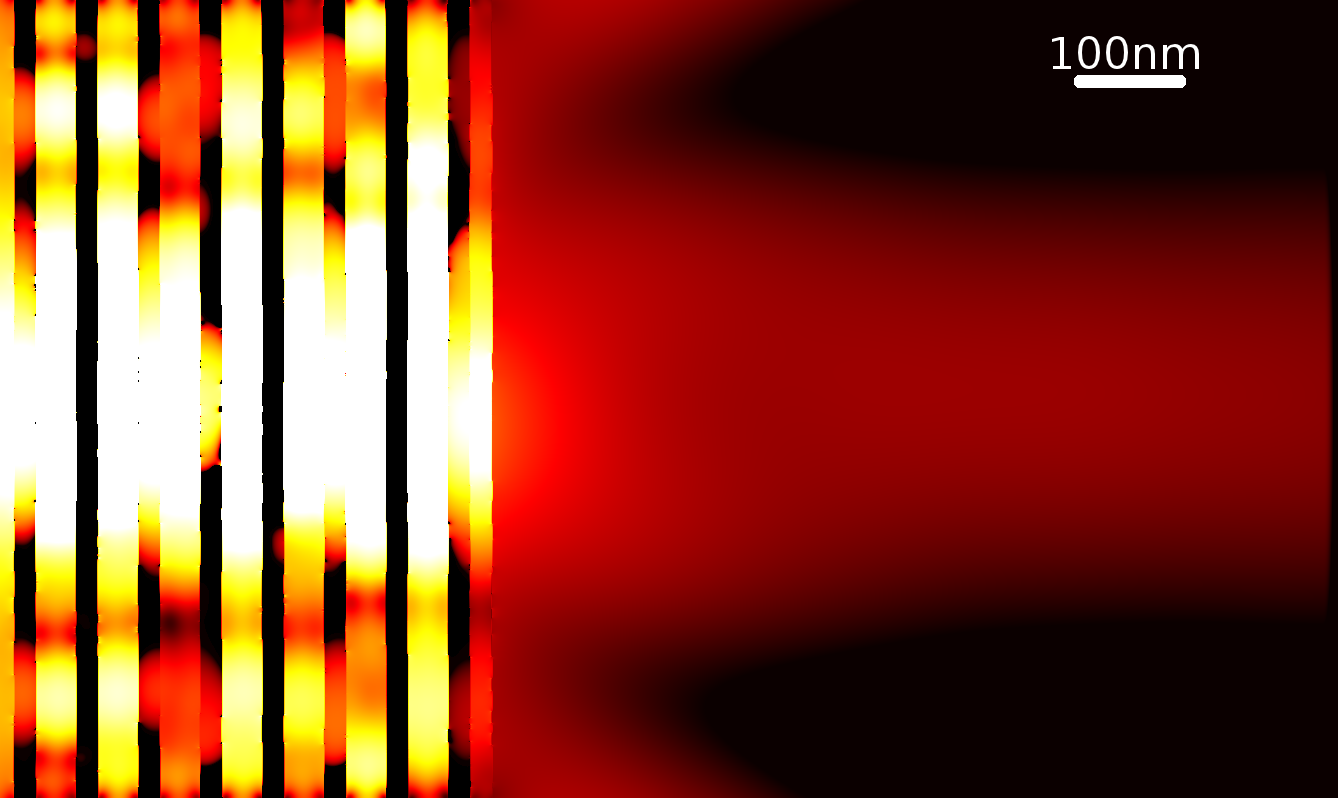
\includegraphics[width=\textwidth]{images/multilayer/oer-rms01.png}
		\caption{$RMS=0.1$~nm}
	\end{subfigure}
	\begin{subfigure}[b]{.45\textwidth}
		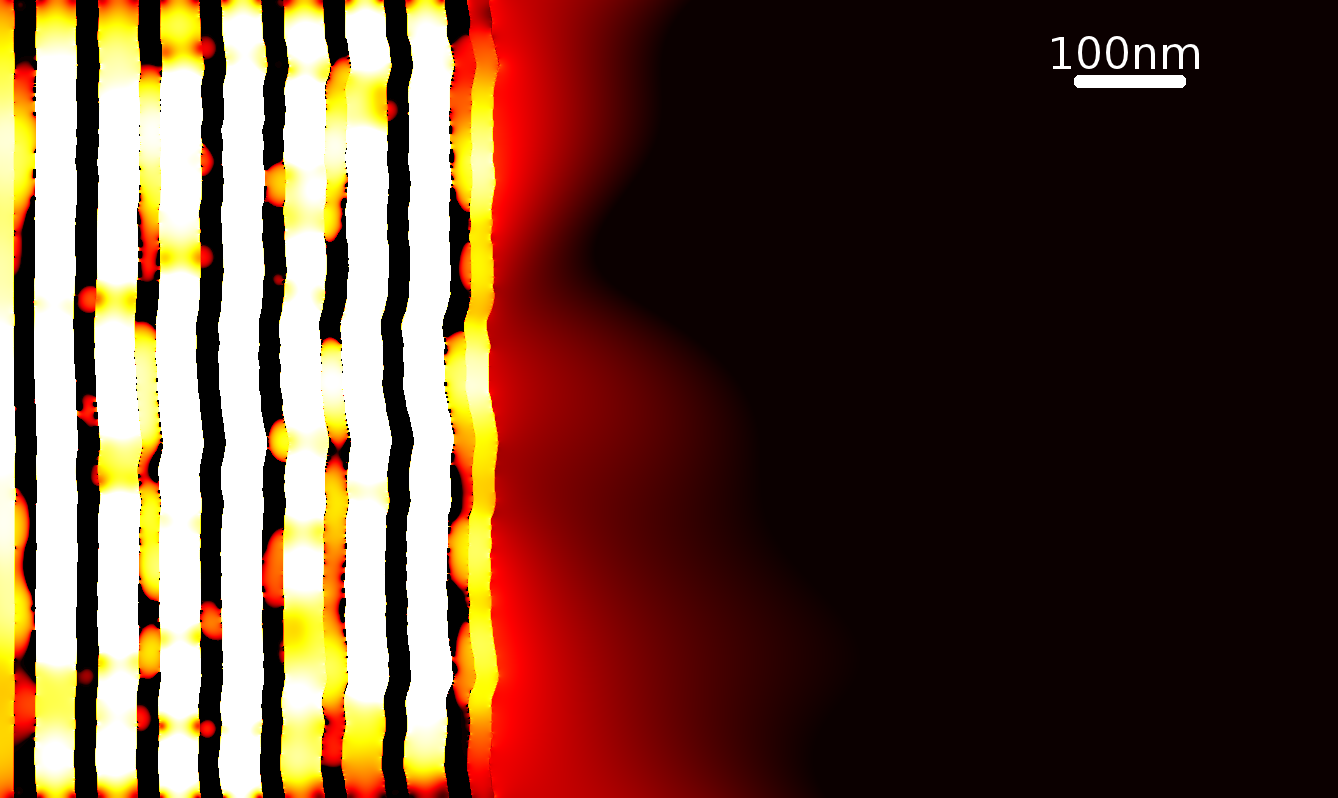
\includegraphics[width=\textwidth]{images/multilayer/oer-rms05.png}
		\caption{$RMS=0.5$~nm}
	\end{subfigure}
	\caption{Wyniki symulacji wielowarstwy o 17 chropowatych granicach ośrodków, z różnymi wartościami RMS charakteryzującymi chropowatość warstw. Na ilustracji (b) obserwujemy znaczne ograniczenie strumienia fali E-M propagującego się w pole dalekie na skutek interferencji wielu fal płaskich losowo zaburzonych przez nierówności.~\cite{pastuszczak2013engineering} }
\end{figure}

Porównanie wyników prac numerycznych dotyczących wpływu chropowatości na współczynnik transmisji, szerokość i kształt PSF oraz zdolność rozdzielczą wielowarstwy wymaga uwzględnienia różnic w metodach zastosowanych w obliczeniach prowadzonych przez różnych autorów. Kluczowym elementem jest sposób generacji powierzchni chropowatej - w niektórych pracach nie jest uwzględniana autokorelacja nierówności \cite{guo2014negative}, w innych wykorzystywane są algorytmy heurystyczne łączące punkty z pomiarów mikroskopowych za pomocą wielomianów sklejanych\footnote{tzw. krzywa B-sklejana, w literaturze polskiej postulowana bywa również nazwa splajn od angielskigo B-spline}\cite{ludwig2012impact}, w innych pracach autorzy opierają się na widmowy rozkładzie gęstości mocy zmiennej losowej\cite{pastuszczak2013engineering}. Przykład powierzchni chropowatej wygenerowanej na podstawie pomiarów z mikroskopu AFM ostatnią meteodą znajduje się na ilustracji \ref{fig:ag30nm-afmgene}.

Niezależnie od zastosowanej metodyki symulacji pola elektromagnetycznego i generacji warstw chropowatych składających się na supersoczewki zbudowane ze struktur MDM wyniki są zgodne. Uzyskanie nadrozdzielczego obrazowania przez omawiane układy  możliwe jest jest jedynie w wielowarstwach o RMS$<1.5$~nm \citep{guo2014negative,stefaniuk2011effect,ludwig2012impact}. Wraz ze wzrostem liczby warstw własności transmisyjne i obrazujące stosu MDM stają się bardziej wrażliwe na chropowatości powierzchni \ref{guo2014negative}. W przypadku stosów składających się z kilkunastu warstw RMS nawet na poziomie $0.5$~nm może uniemożliwić uzyskanie wysokiego współczynnika transmisji, a co za tym idzie praktycznego wykrzystania tego typu soczewek \cite{pastuszczak2013engineering}.




%%%%%%%%Obrazki z publikacji w PLP - wyniki pomoarow afm w 1d i 2d
%%%%%%%%\begin{figure}
%%%%%%%%		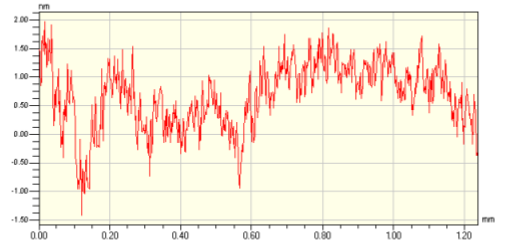
\includegraphics[width=\textwidth]{images/multilayer/plp-afm-chropo-1d.png}\\
%%%%%%%%\end{figure}

%%%%%%%%\begin{figure}
%%%%%%%%		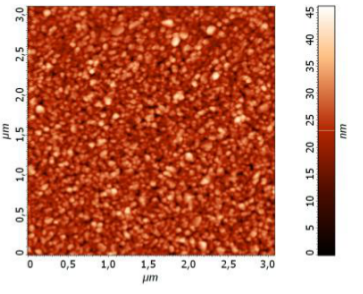
\includegraphics[width=\textwidth]{images/multilayer/plp-afm-chropo.png}\\
%%%%%%%%\end{figure}



